\chapter[~]{Знайомство з базовими можливостями системи КОМПАС-3D}

\textbf{Мета роботи} --- ознайомитись з основними прийомами роботи в програмному пакеті підготовки
конструкторської документації КОМПАС-3D, навчитись виконувати креслення простих деталей на площині.

\section{Короткі теоритичні відомості}

\section{Виконання креслення заданої деталі}

Згідно з варінтом для побудови була задана наступна деталь:

\begin{figure}[!ht]
  \centering
  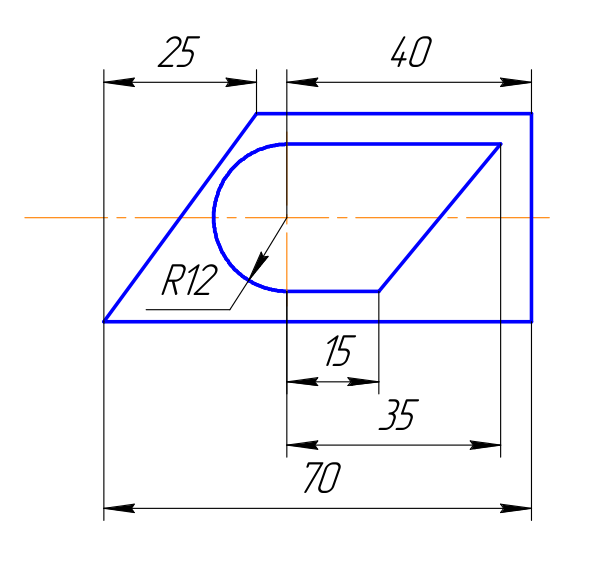
\includegraphics[width=0.9\linewidth]{./images/lab3/target-part.png}
  \caption{Задана деталь для побудови}
  \label{fig:lab3:target_part} 
\end{figure}

\begin{enumerate}[leftmargin=*]
\item За допомогою інструменту ``Прямокутник'' будуємо відповідну фігуру і задаємо необхідні розміри (\ref{fig:lab3:rectangle}).
  \begin{figure}[!ht]
    \centering
    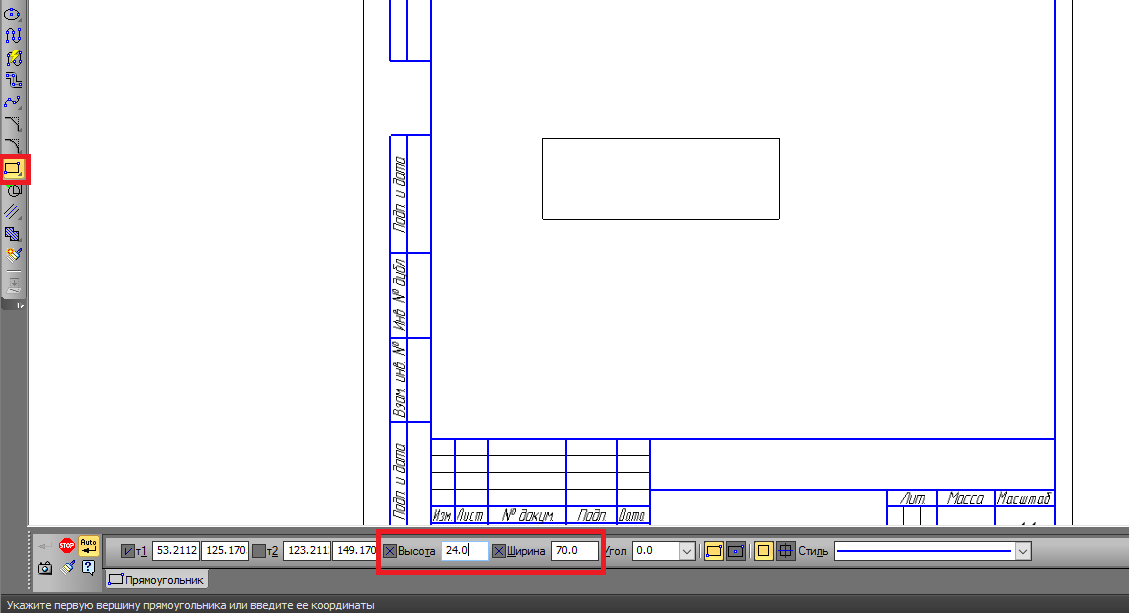
\includegraphics[width=0.9\linewidth]{./images/lab3/step1.png}
    \caption{Застосування інструменту прямокутник}
    \label{fig:lab3:rectangle} 
  \end{figure}

\item За допомогою інструмента ``Автоматичний розмір'' проставляємо розміри деталі (\ref{fig:lab3:dimentions}).
    \begin{figure}[!ht]
      \centering
      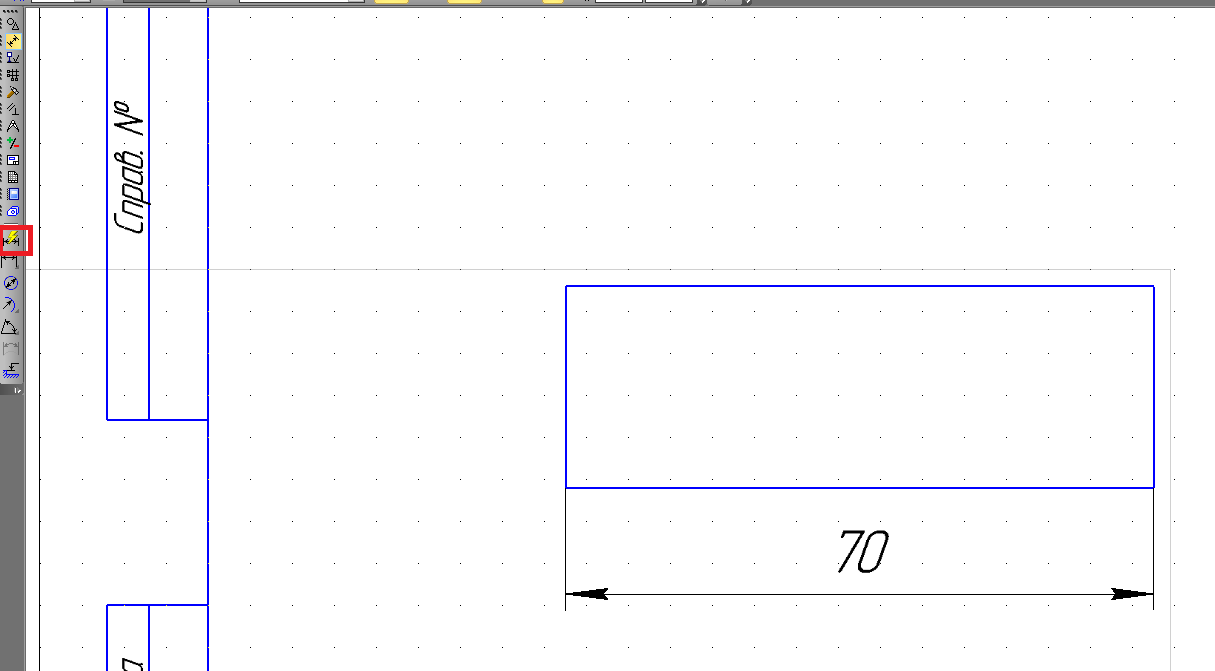
\includegraphics[width=0.9\linewidth]{./images/lab3/step2.png}
      \caption{Застосування інструменту ``Автоматичний розмір''}
      \label{fig:lab3:dimentions} 
    \end{figure}
  \item Видліяємо стоврений прямокутник, і вибираємо в контестному меню (викликається правим кліком
    мишки) пункт ``Зруйнувати'' \textit{(``Разрушить'')}, щоб розділити об’єкт на
    відрізки (\ref{fig:lab3:dismantle}). Після чого формуємо необхідний контур.
    \begin{figure}[!ht]
      \centering
      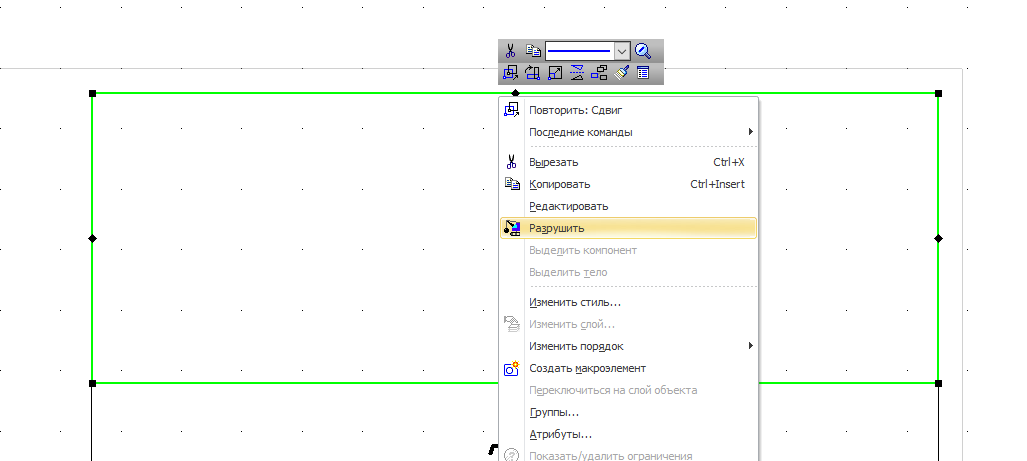
\includegraphics[width=0.9\linewidth]{./images/lab3/step3.png}
      \caption{Застосування інструменту ``Зруйнувати''}
      \label{fig:lab3:dismantle} 
    \end{figure}
  \item За допомогою інструменту ``Дуга'', будуємо дугу з вказаним радіусом (\ref{fig:lab3:step3}).
        \begin{figure}[!ht]
          \centering
          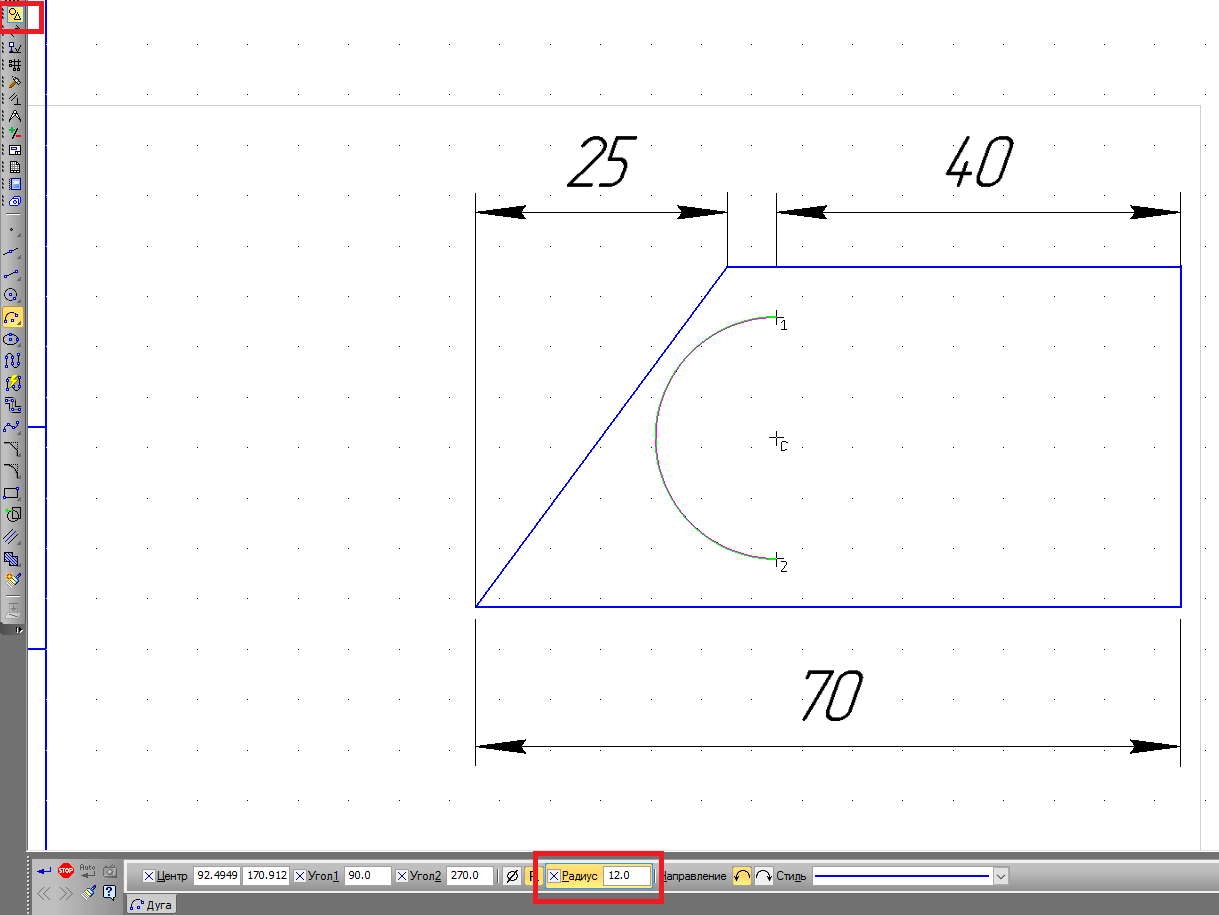
\includegraphics[width=0.9\linewidth]{./images/lab3/step4.png}
          \caption{Застосування інструменту ``Дуга''}
          \label{fig:lab3:step3} 
        \end{figure}

 \item Використовуючи інструмент ``Лінія між двома точками'', будуємо осоьову лінію
   (\ref{fig:lab3:central_line}) та допрацьовуємо внутрішній контур клесленика
   (\ref{fig:lab3:step6}).
   \begin{figure}[!ht]
     \centering
     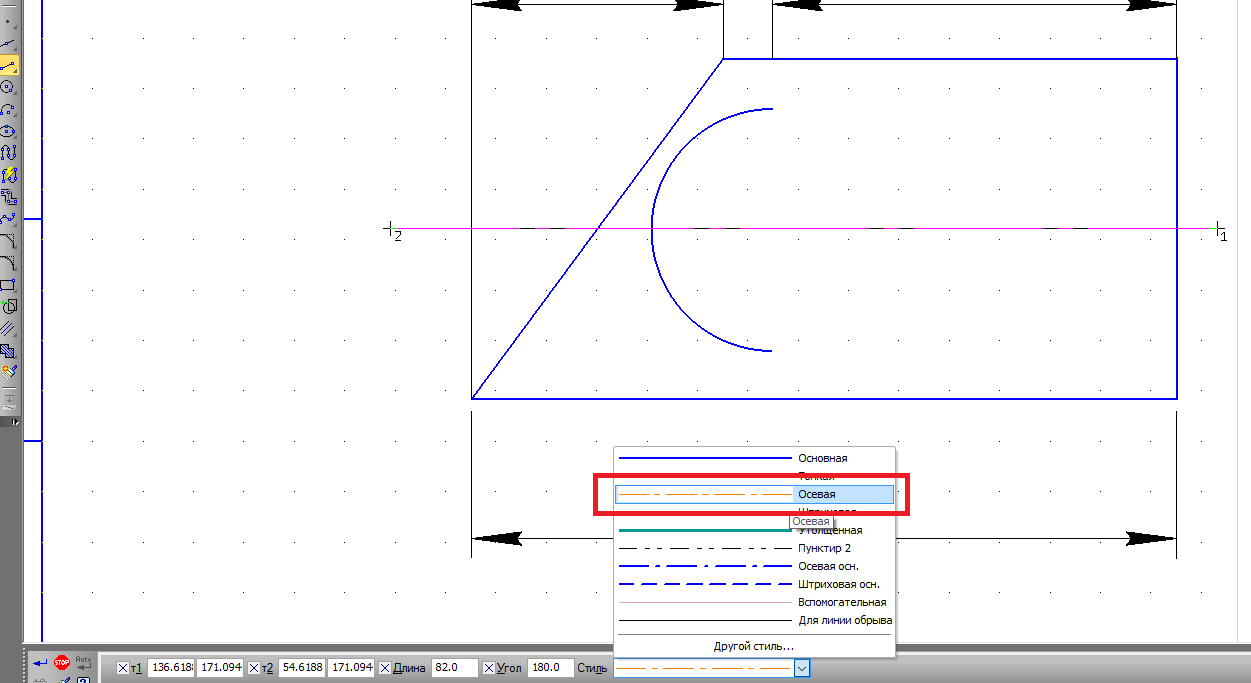
\includegraphics[width=0.9\linewidth]{./images/lab3/step5.png}
     \caption{Застосування інструменту ``Лінія між двома точками''}
     \label{fig:lab3:central_line} 
   \end{figure}
   \begin{figure}[!ht]
     \centering
     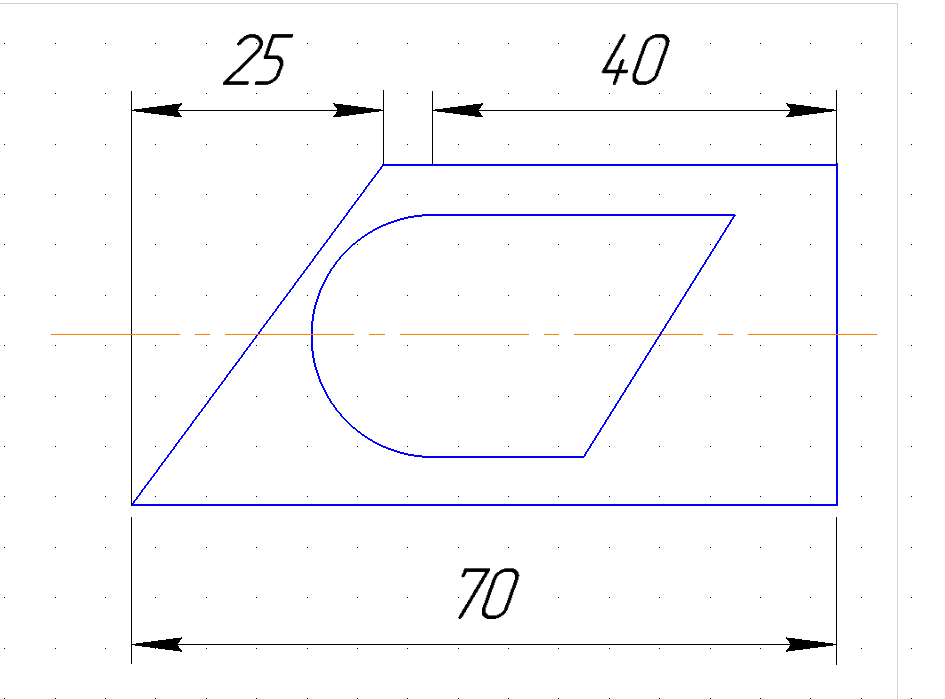
\includegraphics[width=0.9\linewidth]{./images/lab3/step6.png}
     \caption{\label{fig:lab3:step6}}
   \end{figure}

\newpage
 \item Інструментом ``Радіальний розмір'' вказуємо розміри дуги. (\ref{fig:lab3:radial_dimentions}).
   \begin{figure}[!ht]
     \centering
     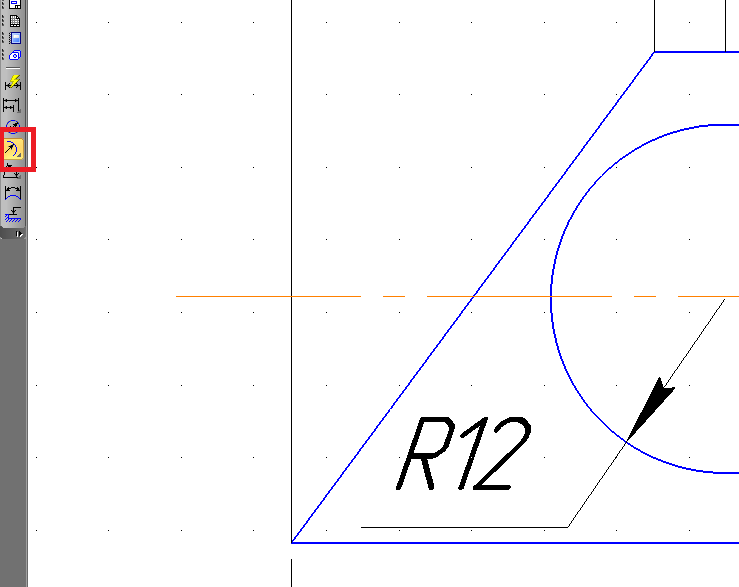
\includegraphics[width=0.9\linewidth]{./images/lab3/step7.png}
     \caption{Застосування інструменту ``Радіальний розмір''}
     \label{fig:lab3:radial_dimentions} 
   \end{figure}

\end{enumerate}

\FloatBarrier
Готовий кресленик навадений на сторінці ____
